\documentclass{article}
\usepackage{amsmath} % import of math elements
\usepackage{mathtools} %import of other math elements
\usepackage{tikz} 
\usetikzlibrary{shapes,positioning,calc} 

%-------------------------------------------------------
% Document information
%-------------------------------------------------------

\title{Robbot project documentation} %Title 

\author{Roberto \textsc{Antoniello}} %author name

\begin{document}
\maketitle % show the title and author and date
%-------------------------------------------------------
%Introduction
%-------------------------------------------------------

\begin{center} In this file I resume how Robbot works with more details than the README file you can find in the repository.
\textbf{Robbot} is a Telegram bot with a bunch of different features. Some of them extend the use of Telegram you usually do, some of them are just funny features I liked to develop.\\
The bot is written in Python and it is running in Python3.9 version at the moment.\end{center}

%-------------------------------------------------------
%First section about configuration file
%-------------------------------------------------------
\section{Configuration file}

The configuration file is the first thing you must check because without it, the bot won't run at all. This file is also well explained in README file in this repository so I won't spend a lot of words on it. \\Essentially you put your keys, additional data and commands' name in the right fields to make the bot work.
\begin{center} $config-example.json \Rightarrow config.json$ \end{center}

\subsection{DB path}
The .db file will be saved in the directory you choose and set in config.json file
\begin{center} $"path-db" \Rightarrow config.json$ \end{center}

\subsection{Super admin data}
In this section we put our Telegram data as super admin(the only one) of the bot. The super admin is able to manage the db changes such as adding users, promote to admin and deleting users/revoke admin powers.\\
This type of user can also modify the value of a few data like the number of uses of commands for a specific user or managing the amount of uses for openai commands of premium users.
\begin{center} $"id-super-admin" \Rightarrow config.json$ \end{center}

\subsection{commands,admin commands and super}
Here we put the name of commands the bot is able to recognize and execute. For example if we don't want to execute the weather we just don't put it on user-commands field. It's the same for admin and super commands.
\begin{center} $"user-commands" \Rightarrow config.json$ \\
               $"admin-commands" \Rightarrow config.json$ \\
               $"super-admin-commands" \Rightarrow config.json$
\end{center}

%-------------------------------------------------------
%Second section about app.py(main)
%-------------------------------------------------------
\section{Main}
\textbf{app.py} is the main source file. It creates the session, it connects with Telegram API using Pyrogram Client class and it's in constant wait for arriving messages.\\
First of all it fetches the information from configuration file, then it starts the connection.\\
While waiting, the bot will ignore any messages it doesn't recognize as a known command. Otherwise if it's a known command, it checks for permission to the user launched that command. If it's a recognized user, the entire message will be managed by a parser function and moved to a specific fetch function written inside \textbf{controller.py}.\\
If a command isn't launched by a registered user, the bot will reply with a default message.
\begin{center} $app.py \xrightarrow{\text{command}} controller.py$ \end{center}

%-------------------------------------------------------
%Third section about the controller
%-------------------------------------------------------
\section{Controller}
Just like in the MVC design pattern, this controller takes the input arriving from the main and it calls the right function in the right source file in $utils$ and $modules$ folders. How it works? \\
There are three dictionaries dedicated to the three types of commands which are as said in before \textbf{(user,admin,super)}. \\The key is the command and the value is the path of function it executes. \\As said in Main section, here we have the fetch command functions matched with the dictionaries mentioned in the previous row. The specific function will return a \textbf{sendMessage} or a \textbf{sendMedia} function and then the main will wait for the next command.
\begin{center} $controller.py \xrightarrow{\text{command fetched}} (modules \ or \ utils)$ \end{center}

\subsection{parser function}
This simple function mentioned in the previous sections takes the input message as argument and it deletes the command at the beginning, returning then just the text "query" that will be sended by the controller to the right module which will manage and execute it.

\subsection{other details}
Inside the controller there is also a small function called \textbf{visualizza} which print the current state of the incoming message on terminal such as a live log.\\ During the execution of this function, the log is also sended as a Telegram message to the super admin private chat, including possible errors/exceptions.  \\

%-------------------------------------------------------
%4th section about the get_config source file
%-------------------------------------------------------
\section{get-config}
this source file contains some support functions that are often used in many situations. The first one return in a variable the content of the configuration file to get the fields easily. \\
The remaining functions are all about Telegram features such as getting information from the json message or renaming for example the \textit{send-message} of \textbf{Pyrogram} to avoid including the decorator in every source file and just call this one by including get-config.
\begin{center} $app.py \xrightarrow{\text{get-config-file()}} running$ \end{center}

%-------------------------------------------------------
%5th section about the sysfunctions source file
%-------------------------------------------------------
\section{sysfunctions}
This file contains functions using directly Telegram features such as the poll function or get-message. It also includes the help function.

\section{Summary till now}
\begin{center} $app.py \xrightarrow{\text{\textbf{get-config-file()}}} running$ \end{center}
\begin{center} $app.py \xrightarrow{\text{\textbf{command}}} controller.py$ \end{center}
\begin{center} $controller.py \xrightarrow{\text{\textbf{command fetched}}} (modules \ or  \ utils)$ \end{center}
\begin{center} $(modules \ or \ utils) \xrightarrow{\text{\textbf{return message or media}}} app.py$ \end{center}
\begin{center} $app.py \xrightarrow{\text{\textbf{waiting for the next command}}} app.py$ \end{center}

%-------------------------------------------------------
%6th section about database
%-------------------------------------------------------
\section{Database}
In this section we'll focus about the database structure. There are several tables linked each other: \textbf{User, Stats, Trivial, Group, OpenAICredit}. \\ \\ \\
The \textbf{User} table saves data of users(Telegram id, first name and username(if it exists otherwise None value), there are also a couple of boolean field to set admin or superadmin rights.\\ \\
The \textbf{Stats} table is linked to the User one by the id field and it saves information about how many times a command is used by every user. \\ \\
The \textbf{Group} table saves chat-id, chat-name and a third string field. This table is used to save a specific command to execute only in specific group chats.\\ \\
The \textbf{Trivial} table is used to manage the score points of the Trivial game developed inside this bot. It's linked to the User table by the id as foreign key. \\ \\
The \textbf{OpenAICredit} table is linked to the User table by the id as foreign key, just used to manage number of uses of premium commands for premium users.

%---Inizializzazione della figura tikz
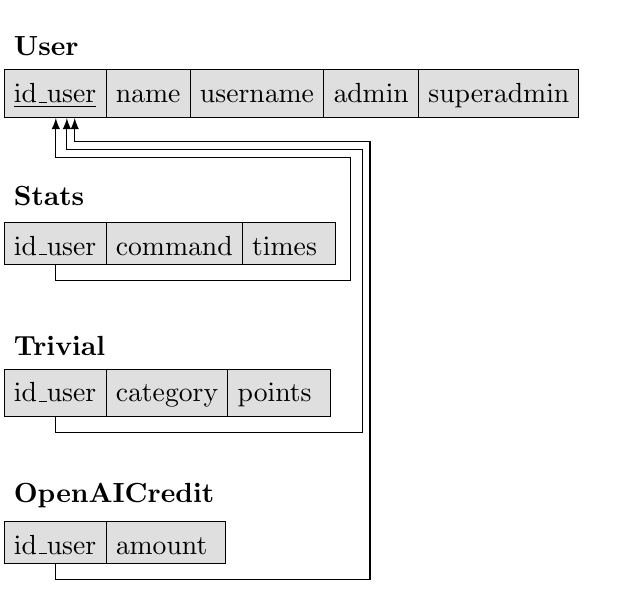
\begin{tikzpicture}[relation/.style={rectangle split, rectangle split parts=#1, rectangle split part align=base, draw, anchor= center, align=center, text height=3mm, text centered}]\hspace*{-0.3cm}

%--figura relativa alla tabella User
\node (usertitle) {\textbf{User}};
\node [relation=5, rectangle split horizontal, rectangle split part fill={lightgray!50}, anchor= north west, below=0.6cm of usertitle.west,anchor=west] (user)
	{\underline{id\_user} 
	\nodepart{two} name
	\nodepart{three} username
	\nodepart{four} admin
	\nodepart{five} superadmin};

%--figura relativa alla tabella Stats
\node [below=1.3cm of user.west,anchor=west] (statstitle) {\textbf{Stats}};
\node [relation=3,rectangle split horizontal, rectangle split part fill ={lightgray!50}, below=0.6cm of statstitle.west,anchor=west] (stats)
	{\nodepart{one} id\_user
	 \nodepart{two} command
	 \nodepart{three} times };

\draw[-latex] (stats.one south) -- ++(0,-0.2) -| ($(stats.one south) + (3.75,0)$) |- ($(user.one south) + (0.25,-0.50)$) -| ($(user.one south) + (0.01,0)$);

%--figura relativa alla tabella Trivial
\node [below=1.3cm of stats.west,anchor=west] (trivialtitle) {\textbf{Trivial}};
\node [relation=3,rectangle split horizontal, rectangle split part fill ={lightgray!50}, below=0.6cm of trivialtitle.west,anchor=west] (trivial)
	{\nodepart{one} id\_user
	 \nodepart{two} category
	 \nodepart{three} points };

\draw[-latex] (trivial.one south) -- ++(0,-0.2) -| ($(trivial.one south) + (3.90,0)$) |- ($(user.one south) + (0.30,-0.400)$) -| ($(user.one south) + (0.15,0)$);

%--figura relativa alla tabella OpenAICredit
\node [below=1.3cm of trivial.west,anchor=west] (openaicredittitle) {\textbf{OpenAICredit}};
\node [relation=2,rectangle split horizontal, rectangle split part fill ={lightgray!50}, below=0.6cm of openaicredittitle.west,anchor=west] (openaicredit)
	{\nodepart{one} id\_user 
	 \nodepart{two} amount };

\draw[-latex] (openaicredit.one south) -- ++(0,-0.2) -| ($(openaicredit.one south) + (4,0)$) |- ($(user.one south) + (0.40,-0.300)$) -| ($(user.one south) + (0.25,0)$);


\end{tikzpicture}

\begin{center}
The \textbf{Group} table isn't linked to any table so it isn't shown in this figure. There's also an additional table called \textbf{TrivialSavedData} but it is standalone like the Group one. It is used to save the current active trivial quiz.\end{center}

\end{document}
